\documentclass[accentcolor=tud9c,colorbacktitle,inverttitle,landscape,german,presentation,t]{tudbeamer}
\usepackage{amstext}
\usepackage{amsmath}
\usepackage{graphicx}
\usepackage{multicol}
\usepackage{mathtools}
\usepackage{subfigure}
\usepackage[ngerman,english]{babel}
\usepackage[utf8]{inputenc}
\usepackage{colortbl}
\usepackage{adjustbox}

\begin{document}

\title{\"Ubung 9 - Gruppe 142}
\subtitle{Visual Computing - 3D-Visualisierung}

\author[Johannes Beck, Christian Eilers, Robin Menzenbach, Martin Steinborn]{Johannes Beck, Christian Eilers, Robin Menzenbach, Martin Steinborn}


\date{\today}

\begin{titleframe}
\end{titleframe}

\section{Aufgabe 1}
	\begin{frame}
		\frametitle{Aufgabe 1: 3D-Daten}
		%TODO
	\end{frame}

\section{Aufgabe 2}
\begin{frame}
	\frametitle{Aufgabe 2: Volumenvisualisierung}
			\begin{itemize}
		\item[a)] %TODO
		\item[b)] %TODO
		\item[c)] %TODO
		\item[d)] %TODO
	\end{itemize}
\end{frame}

\section{Aufgabe 3}
\begin{frame}
	\frametitle{Aufgabe 3: Voronoi-Diagramme}
	\begin{itemize}
	\item[a)] Die Delauney-Triaangulierung des angegebenen Diagramms ist in Abbildung \ref{DelTri} abgebildet. Wie man sehen kann enthält jeder Umkreis lediglich die Punkte desDreiecks selbst. Somit liegt eine korrekte Delauney-Triangulierung vor.
	\begin{figure}
		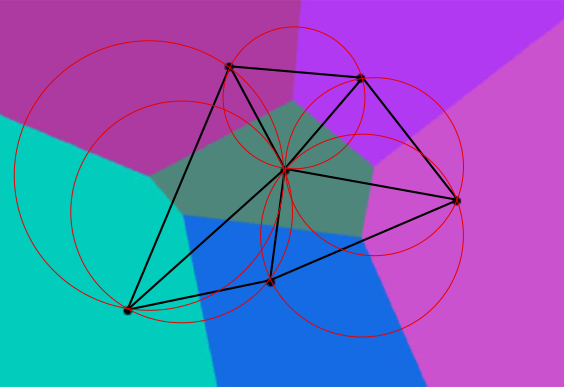
\includegraphics[width = .5\linewidth]{task_3a.png}
		\caption{Delauney-Triangulierung des gegebenen Diagramms}
		\label{DelTri}
	\end{figure}
	\end{itemize} 
\end{frame}
\begin{frame}
	\frametitle{Aufgabe 3: Voronoi-Diagramme}
	\begin{itemize}
	\item[b)] Bei der Erstellung einer Delauney-Triangulierung muss Edge-Flipping angewendet werden, wenn der Umkreis eines Dreiecks einen Punkt eines anderen Dreiecks einschließt. Da dies nicht zulässig ist, wird die gemeinsame Kante der beiden Dreiecke gelöst und die beiden anderen Punkte verbunden. Diesen Vorgang nennt man Edge-Flipping. Ist lediglich eine Punktmenge als ausgangspunkt gegeben, kann diese zu beliebigen Dreiecken(ohne Kantenüberschneidung)  verbunden werden, welche dann mittels Edge-Flipping an Fehlerhaften Stellen in eine Delauney-Triangulierung überführt werden kann. 
	\end{itemize} 
\end{frame}

\section{Aufgabe 4}
\begin{frame}
	\frametitle{Aufgabe 4: Volume Rendering und Marching Cubes}
	\begin{itemize}
	\item[a)] %TODO
	\item[b)] %TODO
	\end{itemize}
\end{frame}

\section{Aufgabe 5}
\begin{frame}
	\frametitle{Aufgabe 5: Marching Squares}
	\begin{itemize}
		\item[a)] %TODO
		\item[b)] %TODO
	\end{itemize}
\end{frame}
\end{document}
